\documentclass[10pt,twocolumn]{article}

\usepackage[margin=0.85in]{geometry}
\usepackage{amsmath,amssymb}
\usepackage{booktabs}
\usepackage{microtype}
\usepackage{xcolor}
\usepackage{tikz}
\usepackage{pgfplots}
\pgfplotsset{compat=1.16}
\usetikzlibrary{arrows.meta,positioning,shapes.geometric,backgrounds,fit,calc}
\usepackage[hidelinks]{hyperref}
\usepackage{caption}
\captionsetup{font=small,labelfont=bf}

% palette (shared with the pillar-UDP papers)
\definecolor{pgood}{RGB}{31,119,80}
\definecolor{pbad}{RGB}{200,40,40}
\definecolor{pnode}{RGB}{38,70,120}
\definecolor{pcell}{RGB}{235,240,248}
\definecolor{pcellb}{RGB}{240,247,240}
\definecolor{pgray}{RGB}{110,110,110}
\definecolor{pmid}{RGB}{210,140,20}

\newcommand{\code}[1]{\texttt{\small #1}}
\newcommand{\Cid}{\code{Cid}}

\tikzset{
  box/.style={rectangle,rounded corners=2pt,draw=pnode,thick,fill=white,
              align=center,font=\footnotesize,inner sep=4pt},
  wide/.style={box,text width=0.86\textwidth},
  half/.style={box,text width=0.40\textwidth},
  seal/.style={box,fill=pcell},
  flow/.style={-{Stealth[length=2mm]},thick,pnode},
  dep/.style={-{Stealth[length=2mm]},thick,pnode},
}

\title{\vspace{-3.5em}\bfseries The Pillar Message Format: One Sealed,
Content-Addressed Envelope for Every Byte Pillar Persists or Transmits}
\author{\normalsize pillar engineering \quad(machine-checked design note)}
\date{\normalsize 2026-09-09}

\begin{document}
\maketitle

\begin{abstract}
\noindent
Pillar today carries what is fundamentally one thing---a signed,
content-addressed record---in three unrelated byte formats: streamdb ops
(hand-rolled length-prefixed \code{SignedSegment}, persisted to an embedded IPFS
node), observability signals (an in-memory timeseries struct, never persisted or
replicated), and libp2p control traffic (per-protocol CBOR, encrypted only by the
transport's Noise session). Three formats mean three serializers, three version
stories, three security postures---and observability gets none of the durability,
content-addressing, or replication streamdb already has. We unify them behind a
single record: the \textbf{\code{PillarMessage}}, a version-stamped envelope whose
payload is AEAD-sealed to the owning \emph{cell} and addressed by the SHA2-256
multihash of its canonical CBOR encoding. The crux is a \emph{convergent} content
seal: the nonce is derived (HKDF) from the cell key and the content address of the
plaintext, so identical bodies produce identical ciphertext and hence an identical
\Cid{} on every node---dedup, IPFS convergence, and Merkle roots all survive
encryption---while distinct plaintexts never share a nonce (AEAD-safe). streamdb
ops, observability signals, and every control message become body variants of the
one envelope, owned by a new shared crate \code{pillar-wire} onto which streamdb,
observability, and net all depend \emph{down}. On the wire the envelope rides a
pillar-UDP datagram sealed under a portable, cell-minted session key (companion
paper), or a QUIC/TCP connection under the transport's own TLS; the content seal
is transport-agnostic and holds either way, so no transport ever sees plaintext.
Per Pillar's method \#1, this is the design of record and the implementation is
TLA\textsuperscript{+}-gated: \code{OneRecordFormat}, \code{ContentAddressStable},
\code{DedupUnderEncryption}, \code{CellConfidential}, and
\code{NoNonceReuseAcrossDistinctPlaintext} must be green under TLC before any Rust.
\end{abstract}

\section{Motivation}
The three formats Pillar uses today for one logical object---a signed,
content-addressed record---are: \textbf{streamdb ops},
\code{SignedSegment\{bytes,signer,signature,visibility\}}, a hand-rolled
length-prefixed wire form addressed by \code{Cid=content\_address(to\_wire())} and
persisted through \code{ContentStore}/\code{IpfsBackend} onto Pillar's embedded
IPFS node; \textbf{observability signals},
\code{Signal\{id,kind,payload,labels,expiry\}}, held only in an in-memory
\code{TimeseriesStore}, never persisted, never on the wire; and \textbf{libp2p
control traffic}, per-protocol CBOR request/response types plus gossipsub
event-log messages, each its own struct, encrypted only by the libp2p Noise
session at the transport layer.

Three formats mean three serializers, three version stories, three security
postures, and---critically---observability signals get \emph{none} of the
durability, content-addressing, or replication that streamdb ops already have. The
five signal kinds (metric/log/trace/profile/metadata) are already specified to
ride ``IPFS (durable signed segments/backfill) $+$ streaming-DB tip $\dots$ no
parallel store, no second authority'' (ROI Priority~3). This paper makes that
literal by giving signals the \emph{same} record type streamdb ops use.

\paragraph{Thesis.} There is exactly one Pillar record on the wire and on disk:
the \code{PillarMessage}, a version-stamped envelope carrying a sealed,
content-addressed payload, of which streamdb ops, observability signals, and every
control message are variants. It is (1)~\textbf{content-addressed}---its \Cid{} is
the SHA2-256 multihash of its canonical encoding, identical on every node;
(2)~\textbf{sealed to the cell}---the payload is AEAD-encrypted under the cell
group key, \emph{convergently} so the \Cid{} is stable across nodes despite
encryption; (3)~\textbf{version-stamped}---an independently incrementable surface
version, per the ROI versioning spine; and (4)~\textbf{the payload of a pillar-UDP
datagram} (fallback QUIC, then TCP$+$TLS).

\begin{figure*}[t]
\centering
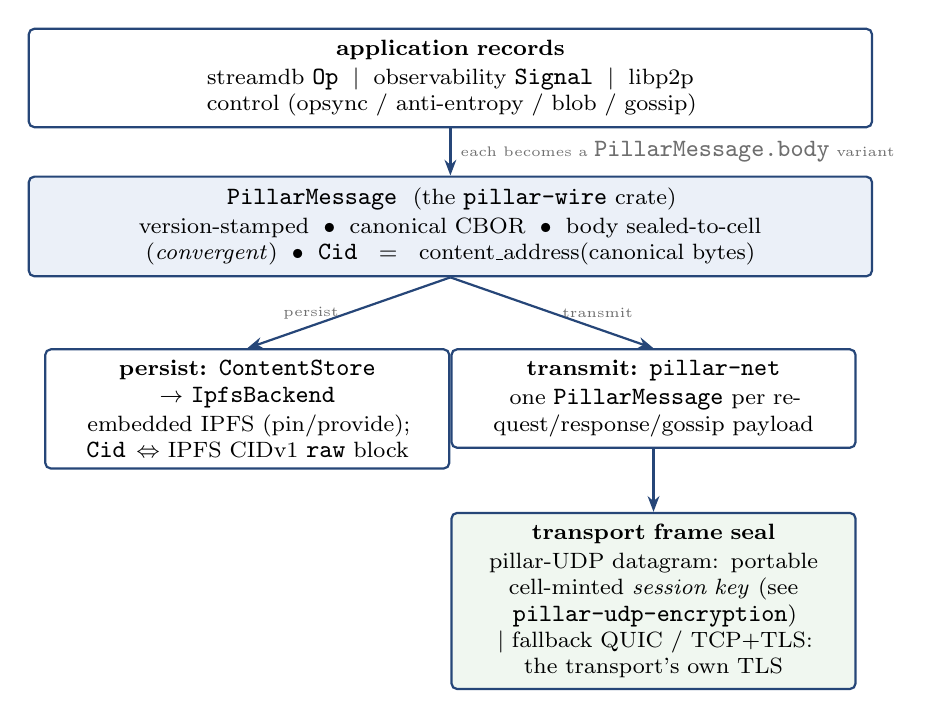
\begin{tikzpicture}[node distance=5mm]
  \node[wide] (app) {\textbf{application records}\\[1pt]
     streamdb \code{Op} \;$\mid$\; observability \code{Signal} \;$\mid$\;
     libp2p control (opsync / anti-entropy / blob / gossip)};
  \node[wide,below=6mm of app,fill=pcell] (pm) {\textbf{\code{PillarMessage}}
     \ (the \code{pillar-wire} crate)\\[1pt]
     version-stamped \;$\bullet$\; canonical CBOR \;$\bullet$\;
     body sealed-to-cell (\emph{convergent}) \;$\bullet$\;
     $\Cid{}=\mathrm{content\_address}(\text{canonical bytes})$};
  \draw[flow] (app) -- node[right,font=\tiny,pgray]
     {each becomes a \code{PillarMessage.body} variant} (pm);
  \node[half,below left=9mm and 0mm of pm.south] (store)
     {\textbf{persist:} \code{ContentStore} $\to$ \code{IpfsBackend}\\[1pt]
      embedded IPFS (pin/provide); $\Cid{}\Leftrightarrow$ IPFS CIDv1 \code{raw} block};
  \node[half,below right=9mm and 0mm of pm.south] (net)
     {\textbf{transmit:} \code{pillar-net}\\[1pt]
      one \code{PillarMessage} per request/response/gossip payload};
  \draw[flow] (pm.south) -- node[left,font=\tiny,pgray]{persist} (store.north);
  \draw[flow] (pm.south) -- node[right,font=\tiny,pgray]{transmit} (net.north);
  \node[half,below=8mm of net,fill=pcellb] (xport)
     {\textbf{transport frame seal}\\[1pt]
      pillar-UDP datagram: portable cell-minted \emph{session key}
      (see \code{pillar-udp-encryption})\\
      $\mid$ fallback QUIC / TCP$+$TLS: the transport's own TLS};
  \draw[flow] (net.south) -- (xport.north);
\end{tikzpicture}
\caption{\textbf{Layering.} Every application record becomes the body of one
\code{PillarMessage}; the envelope is content-addressed and cell-sealed once, then
either persisted as an IPFS block or transmitted by \code{pillar-net}. The body
seal travels \emph{with} the record (an on-disk block is already sealed; a bitswap
peer outside the cell cannot read it), so it is independent of, and composes with,
the transport frame seal below---which is the pillar-UDP session key on pillar-UDP
and the transport's native TLS on QUIC/TCP. A datagram to a cell therefore carries
a cell-sealed body inside a session-key-sealed datagram: double-sealed, each layer
independent.}
\label{fig:layering}
\end{figure*}

\section{Two seals, deliberately}
The design has two distinct seals because they protect different things
(Table~\ref{tab:seals}). The \textbf{content seal} is on \code{PillarMessage.body},
keyed by the cell group key with a \emph{deterministic} (convergent) nonce; it
gives confidentiality at rest, a stable \Cid{}, and dedup. The \textbf{transport
frame seal} is on the pillar-UDP datagram, keyed by a portable cell-minted session
key with a collision-free nonce; it protects on-wire framing. On QUIC/TCP the
transport's native TLS plays the second role instead.

\begin{table}[t]
\footnotesize
\setlength{\tabcolsep}{3.5pt}
\begin{tabular}{@{}p{0.15\columnwidth}p{0.36\columnwidth}p{0.40\columnwidth}@{}}
\toprule
 & \textbf{content seal} & \textbf{transport frame seal} \\
\midrule
layer     & \code{PillarMessage.body} & pillar-UDP datagram \\
recipient & the cell & the cell (any member) \\
key       & cell group key (symmetric) & portable cell-minted session key $K_s$ \\
nonce     & \textbf{deterministic} (convergent) & collision-free (convergent / sender-partitioned) \\
purpose   & confidentiality at rest $+$ stable \Cid{} $+$ dedup & confidentiality of transport framing \\
\bottomrule
\end{tabular}
\caption{The two seals protect different things and compose. The content seal is
transport-agnostic and travels with the record; the transport frame seal is
pillar-UDP-specific (its portable session key is the subject of the companion
paper \code{pillar-udp-encryption}). On QUIC/TCP the transport's TLS supplies the
frame seal instead.}
\label{tab:seals}
\end{table}

\section{\code{pillar-wire}: the shared substrate crate}
Both streamdb and observability \textbf{depend down} onto one shared crate rather
than sideways onto each other; that crate is \code{pillar-wire}---the common home
for the wire/persistence primitives currently trapped inside \code{pillar-streamdb}
(named because the \emph{same} bytes go on the wire and to disk; the deliberately
broad ``widely used substrate'' crate preferred over a scatter of opaque
micro-crates). It owns \code{PillarMessage} (the envelope enum $+$ its canonical
CBOR codec $+$ \Cid{} derivation), the content seal
(\code{cell\_seal\_convergent}/\code{cell\_open\_convergent}, wrapping
\code{pillar-crypto}), and---\emph{moved down} from \code{pillar-streamdb}---
\code{SignedSegment}, \code{Cid}, \code{HeadRecord}, \code{Visibility},
\code{ContentStore}, and the \code{IpfsBackend} trait. The dependency direction is
strictly downward, no cycles:
\begin{center}\footnotesize
\code{pillar-streamdb}, \code{pillar-observability}, \code{pillar-net}
\ $\to$\ \code{pillar-wire}\ $\to$\
\code{pillar-crypto}, \code{pillar-core}, \code{pillar-ipfs}.
\end{center}
\code{pillar-wire} must \emph{not} depend on \code{pillar-net} (net uses the
envelope, not the reverse) nor on the two crates that depend on it.

\section{The envelope}
The one record---persisted and transmitted---and the body it seals:
\begin{quote}\footnotesize\ttfamily
struct PillarMessage \{\\
\hspace*{1.2em}version\ \ \ \ \ : SurfaceVersion\\
\hspace*{1.2em}signer\ \ \ \ \ \ : SigningPublicKey\\
\hspace*{1.2em}signature\ \ \ : Signature\ // over body\_sealed\\
\hspace*{1.2em}visibility\ \ : Visibility\ // DHT reach\\
\hspace*{1.2em}cell\ \ \ \ \ \ \ \ : CellId\ // which group key opens it\\
\hspace*{1.2em}body\_sealed : Ciphertext\ // convergent AEAD\\
\}\\[3pt]
enum Body \{\ // what body\_sealed decodes to\\
\hspace*{1.2em}StreamOp(StreamOpBody),\ // CRDT op-log\\
\hspace*{1.2em}Signal(SignalBody),\ \ \ // one of 5 kinds\\
\hspace*{1.2em}Control(ControlBody),\ \ // opsync/AE/blob/gossip\\
\}
\end{quote}

\paragraph{Canonical encoding.} The envelope and \code{Body} are encoded with
\textbf{deterministic CBOR} (RFC~8949 \S4.2.1: sorted map keys, definite lengths,
shortest-int)---CBOR because \code{pillar-net} already uses
\code{request\_response::cbor}, and determinism because the \Cid{} is a hash of
these bytes, so two nodes MUST produce byte-identical encodings for one logical
record or content-addressing breaks. This replaces streamdb's hand-rolled
\code{to\_wire}; \code{SignedSegment::to\_wire}/\code{from\_wire} become the
\code{version=1} read-compatibility path (\S\ref{sec:compat}).

\paragraph{Content address.}
$\Cid{}=\mathrm{content\_address}(\mathrm{canonical\_cbor}(\code{PillarMessage}))$,
the existing \code{pillar-crypto} SHA2-256 multihash---the same function streamdb
and observability already share, and the same multihash inside an IPFS CIDv1
\code{raw} block. Signing is over \code{body\_sealed} (the ciphertext), so
signature verification needs no cell key, decryption needs the cell key, and both
are independent of the \Cid{}.

\section{Convergent content seal (the crux)}\label{sec:seal}
The promise is: \emph{the encryption recipient is the cell; any cell node can
decrypt; the \Cid{} is the same across nodes; we deliver BOTH dedup AND
encryption.} Na\"ively this is impossible---\code{pillar-crypto::seal\_symmetric}
draws a \emph{random} nonce, so the same signal sealed on two nodes yields
different ciphertext, a different \Cid{}, and no dedup. We therefore add a
\emph{convergent} seal:
\begin{align*}
\mathit{nonce} &= \mathrm{HKDF}\big(\text{key}{=}\mathit{cell\_group\_key},\\[-1pt]
 &\quad \text{info}{=}\text{``}\dots\text{/convergent-nonce/v1''}\|\mathit{domain},\\[-1pt]
 &\quad \text{ikm}{=}\mathrm{content\_address}(\mathit{plaintext})\big)[..n]\\
\mathit{ct} &= \mathrm{AEAD\_seal}(\mathit{cell\_group\_key},\mathit{nonce},
   \mathit{plaintext},\\[-1pt]
 &\qquad \text{aad}{=}\mathit{envelope\_header})
\end{align*}
Its properties: \textbf{deterministic}---the nonce is a pure function of (cell key,
plaintext), so identical body $+$ identical cell key $\Rightarrow$ identical
ciphertext $\Rightarrow$ identical \Cid{} on every node (the streamdb CRDT
idempotence guarantee, now for sealed content); \textbf{confidential}---recovered
only with the cell group key, itself sealed to each member by the existing
\code{distribute\_group\_key} (X25519 sealed-box), so a non-member or bitswap peer
holds only ciphertext; \textbf{nonce-safe}---reuse happens \emph{only} for
identical plaintext (which produces identical ciphertext anyway---the intended
dedup), never across distinct plaintexts, because the nonce binds
$\mathrm{content\_address}(\mathit{plaintext})$; and an \textbf{equality leak},
accepted and documented---convergent encryption reveals that two sealed records are
byte-identical (that is \emph{how} dedup works), a property scoped to the cell
confidentiality boundary, with the \code{domain} input separating record classes
so equality never leaks across classes. This is the one genuinely new
cryptographic primitive the refactor introduces, and it earns its own TLC
obligations and \code{pillar-crypto} contract tests.

\section{Transport}\label{sec:transport}
The envelope's on-wire encryption depends on the transport, and there are exactly
two cases. \textbf{pillar-UDP} (a bare datagram substrate) supplies its own frame
encryption keyed by a \textbf{portable, cell-minted session key}---established by a
\emph{cell-as-KDC} scheme distributed over streamdb, with the session key derived
deterministically from the client's ephemeral key against the cell static key. It
replaces the libp2p Noise upgrade; it is neither handshakeless-per-peer nor a
per-pair Noise session---the key is portable across every cell node, so any
ingress/relay can carry the session. The complete scheme (packet flow, key
derivation, anonymous handling, revocation/GC, the forward-secrecy tradeoff) is its
own design of record, the companion paper \code{pillar-udp-encryption},
TLA\textsuperscript{+}-gated by \code{specs/PillarUdpEncryption.tla}.
\textbf{QUIC/TCP} (the fallbacks) bring their own \textbf{TLS~1.3}; the pillar-UDP
scheme does not apply there. The selection order is pillar-UDP $\to$ QUIC $\to$
TCP$+$TLS, and because the body is \emph{already} cell-sealed (\S\ref{sec:seal}),
even the fallback transports never see plaintext application content. All libp2p
control messages ride \emph{inside} the envelope, exactly like ops and signals;
pillar-UDP sits beneath IPFS in the stack. Removing the Noise upgrade is a
deliberate, \emph{breaking} change, safe only behind the versioning spine
(\S\ref{sec:compat}).

\section{Compatibility \& versioning}\label{sec:compat}
Per the ROI versioning spine (independent per-surface stamps, $N{-}1$ window): the
\textbf{envelope version} (\code{PillarMessage.version}) is \code{v1}$=$ the legacy
\code{SignedSegment} length-prefixed form (read-compat), \code{v2}$=$ this
canonical-CBOR convergent envelope; the \textbf{pillar-UDP protocol version} bumps
for the Noise$\to$session-key cutover; and the \textbf{sealed-artifact version} is
the convergent-seal algorithm tag (its KDF carries a \code{"/v1"} \code{info} so a
future scheme coexists). A stamped-but-unknown \emph{future} version is rejected
\emph{distinctly} from a parse error, so a node one version ahead is refused
cleanly, not silently mis-read. Migration is read-through: a \code{v1} \Cid{} stays
valid, new writes are \code{v2}, and the content-addressed store lets both coexist
by construction---no history rewrite.

\section{What changes, concretely}
New crate \code{pillar-wire} (envelope $+$ codec $+$ convergent seal $+$ the
primitives moved down from streamdb). \code{pillar-crypto} gains
\code{cell\_seal\_convergent}/\code{cell\_open\_convergent} alongside the existing
random-nonce \code{seal\_symmetric}. \code{pillar-streamdb} \code{Op}/\code{OpLog}
payloads become \code{StreamOp} bodies; persistence re-exports \code{pillar-wire}'s
\code{ContentStore} (no CRDT/Merkle change). \code{pillar-observability}
\code{Signal}s become \code{Signal} bodies, each persisted as a sealed,
content-addressed IPFS block via \code{ContentStore}, with cross-node backfill on
the same substrate as streamdb. \code{pillar-net} makes every payload a
\code{PillarMessage}, drops the pillar-UDP Noise upgrade for the portable session
key, and turns the per-protocol CBOR types into \code{ControlBody} variants.

\section{Invariants (before any Rust)}
The design is TLA\textsuperscript{+}-gated (method \#1). It refines/extends the
existing \code{versioning-compat-migration-spec} and \code{ObsIngestionSubstrate};
Table~\ref{tab:inv} lists the envelope/content obligations, all green under TLC in
\code{specs/PillarMessageFormat.tla}. The transport-frame obligations (portable
session-key convergence, cell-signed session records, anonymous-as-unattested
policy, replay-via-dedup, revoked-key erasure) are proven separately in
\code{specs/PillarUdpEncryption.tla}.

\begin{table}[t]
\footnotesize
\setlength{\tabcolsep}{4pt}
\begin{tabular}{@{}p{0.36\columnwidth}p{0.58\columnwidth}@{}}
\toprule
\textbf{Invariant} & \textbf{Guarantee} \\
\midrule
\code{OneRecordFormat} & every persisted/transmitted byte is a \code{PillarMessage} \\
\code{ContentAddress\-Stable} & \Cid{} is a deterministic function of the logical record, equal across nodes despite sealing \\
\code{DedupUnder\-Encryption} & identical sealed records collapse to one \Cid{}/one block \\
\code{CellConfidential} & only a cell-key holder recovers \code{Body}; a non-member/bitswap peer gets ciphertext only \\
\code{NoNonceReuseAcross\-DistinctPlaintext} & convergent content nonces collide only for identical plaintext \\
\code{Negotiation\-Refuses\-Incompatible}, \code{Rolling\-Coexistence} & envelope, pillar-UDP, and seal versions bump independently; a mixed-version (incl.\ Noise-era) swarm never mis-frames or partitions \\
\bottomrule
\end{tabular}
\caption{TLA\textsuperscript{+} obligations of \code{PillarMessageFormat.tla} (the
transport-agnostic envelope $+$ convergent content seal $+$ version negotiation).}
\label{tab:inv}
\end{table}

\section{Resolved design points}
\textbf{Anonymous-session transport crypto}---\emph{resolved}: anonymous clients
use the \emph{exact same} pillar-UDP session-key scheme; anonymity is a
\emph{policy} property, not a crypto scheme (an anonymous key is cryptographically
equivalent to a user/node key and subject to the same WoT/RBAC checks; lacking
attestations, the cell withholds sensitive data and privileged operations by
default-deny). \textbf{Transport forward secrecy}---\emph{accepted tradeoff}: the
portable session key is derivable under the cell static key, so transport FS bounds
to cell-key security plus erase-on-revoke---the same price the content seal already
pays, with per-session ephemeral FS deliberately traded for cross-node
portability. \textbf{Convergent-encryption equality leak (\S\ref{sec:seal})}---
accepted as the mechanism of dedup, scoped to the cell boundary, flagged so it is
an explicit reviewed acceptance rather than an accident. The first two are detailed
in \code{pillar-udp-encryption}.

\begin{thebibliography}{9}
\bibitem{cbor} C.~Bormann and P.~Hoffman, \emph{Concise Binary Object
  Representation (CBOR)}, RFC~8949, 2020.
\bibitem{ipfs} J.~Benet, \emph{IPFS---Content Addressed, Versioned, P2P File
  System}, arXiv:1407.3561, 2014.
\bibitem{hkdf} H.~Krawczyk, \emph{Cryptographic Extraction and Key Derivation:
  The HKDF Scheme}, CRYPTO, 2010.
\bibitem{tlaplus} L.~Lamport, \emph{Specifying Systems}, Addison-Wesley, 2002.
\end{thebibliography}

\end{document}
